\documentclass[border=2pt]{standalone}
\usepackage{tikz}
\usetikzlibrary{arrows.meta,chains,%
                    decorations.pathreplacing}
\usetikzlibrary{matrix,positioning,arrows.meta,arrows}

\tikzset{
mymat/.style={
  matrix of nodes,
  nodes in empty cells,
  text height=2.5ex,
  text depth=0.75ex,
  text width=3.25ex,
  align=center,
  column sep=-\pgflinewidth
  }
}
\tikzset{
  rows/.style 2 args={
    sub@rows/.style={row ##1 column #2/.style={nodes={rectangle,draw=black}}},
    sub@rows/.list={#1}
  },
  box/.style 2 args={
    sub@box/.style={rows={#1}{##1}},
    sub@box/.list={#2}
  }
}
\begin{document}

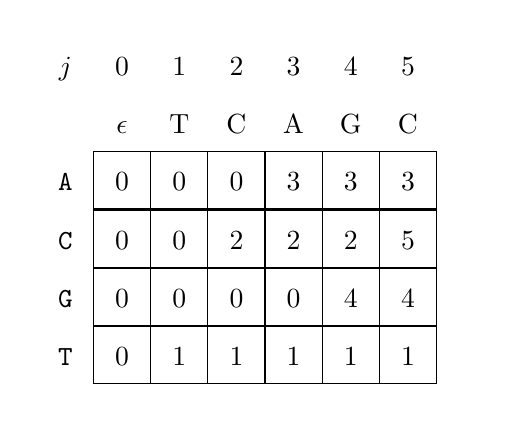
\begin{tikzpicture}[>=latex]
\matrix[mymat,anchor=west,
    box={3, 4, 5, 6}{2, 3, 4, 5, 6, 7}]
at (0,0) 
(mat1)
{ 
  $j$ & 0 & 1 & 2 & 3 & 4 & 5 \\
   & $\epsilon$ & T & C & A & G & C & \\
  $\texttt{A}$ & 0 & 0 & 0 & 3 & 3 & 3 \\
  $\texttt{C}$ & 0 & 0 & 2 & 2 & 2 & 5 & \\
  $\texttt{G}$ & 0 & 0 & 0 & 0 & 4 & 4 & \\
  $\texttt{T}$ & 0 & 1 & 1 & 1 & 1 & 1 & \\ };
\end{tikzpicture}

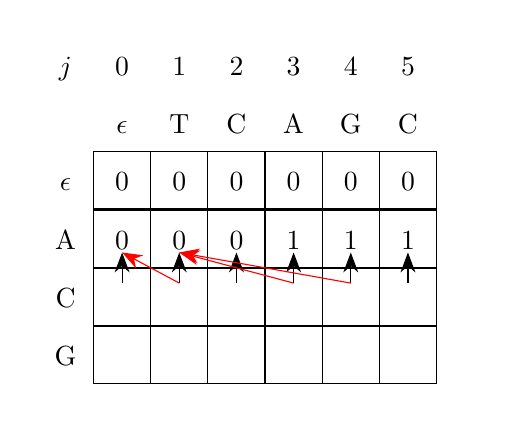
\begin{tikzpicture}[>=latex]
\matrix[mymat,anchor=west,
    box={3, 4, 5, 6}{2, 3, 4, 5, 6, 7}]
at (0,0) 
(mat1)
{ 
  $j$ & 0 & 1 & 2 & 3 & 4 & 5 \\
   & $\epsilon$ & T & C & A & G & C & \\
  $\epsilon$ & 0 & 0 & 0 & 0 & 0 & 0 &\\
  A & 0 & 0 & 0 & 1 & 1 & 1 \\
  C &  &  &  &  &  &  & \\
  G &  &  &  &  &  &  & \\
};

\begin{scope}
\coordinate(start) at([yshift=5pt]mat1-5-2.center);
\coordinate(end) at([yshift=-5pt]mat1-4-2.center);

\draw[-{Stealth[scale=1.5]}] (start) -- (end);
\end{scope}

\begin{scope}
\coordinate(start) at([yshift=5pt]mat1-5-3.center);
\coordinate(end) at([yshift=-5pt]mat1-4-3.center);
\coordinate(end2) at([yshift=-5pt]mat1-4-2.center);

\draw[-{Stealth[scale=1.5]}] (start) -- (end);
\draw[-{Stealth[scale=1.5]}, red] (start) -- (end2);
\end{scope}

\begin{scope}
\coordinate(start) at([yshift=5pt]mat1-5-4.center);
\coordinate(end) at([yshift=-5pt]mat1-4-4.center);

\draw[-{Stealth[scale=1.5]}] (start) -- (end);
\end{scope}

\begin{scope}
\coordinate(start) at([yshift=5pt]mat1-5-5.center);
\coordinate(end) at([yshift=-5pt]mat1-4-5.center);
\coordinate(end2) at([yshift=-5pt]mat1-4-3.center);

\draw[-{Stealth[scale=1.5]}] (start) -- (end);
\draw[-{Stealth[scale=1.5]}, red] (start) -- (end2);
\end{scope}

\begin{scope}
\coordinate(start) at([yshift=5pt]mat1-5-6.center);
\coordinate(end) at([yshift=-5pt]mat1-4-6.center);
\coordinate(end2) at([yshift=-5pt]mat1-4-3.center);

\draw[-{Stealth[scale=1.5]}] (start) -- (end);
\draw[-{Stealth[scale=1.5]}, red] (start) -- (end2);
\end{scope}

\begin{scope}
\coordinate(start) at([yshift=5pt]mat1-5-7.center);
\coordinate(end) at([yshift=-5pt]mat1-4-7.center);

\draw[-{Stealth[scale=1.5]}] (start) -- (end);
\end{scope}

\end{tikzpicture}

\end{document}